\chapter{Methods}

The pipeline of this work relies on the following steps:
\begin{enumerate}
    \item Library selection;
    \item Fingerprints generation;
    \item ML model selection;
    \item Iterative algorithm building.
\end{enumerate}
All steps will be considered in detail in this chapter.
\section{Dataset selection}

\acrshort{smiles} of drug-like molecules from ZINC20 library were taken as a dataset for this work with following rules: $200\ <\ \text{MW}\ <\ 500$, $\text{logP} < 5$.
The distribution of number of compounds on their molecular weight and log P is showed on  Fig.\ref{zinc}.

\begin{figure}[H]
    \centering
    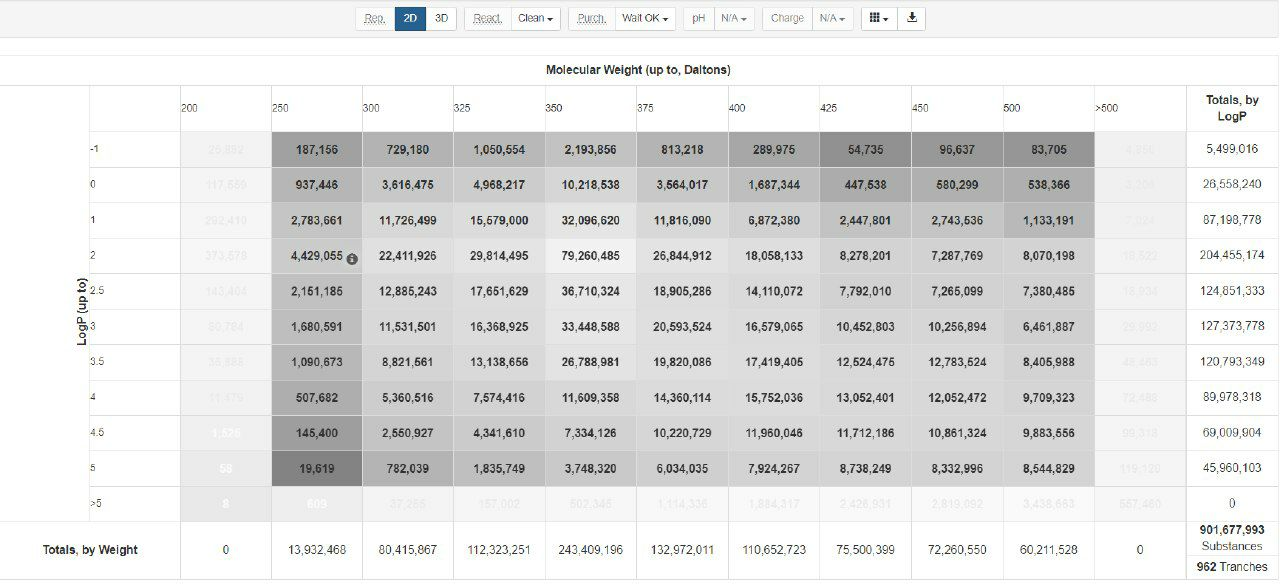
\includegraphics[scale=0.35]{Images/zinc.jpg}
    \caption{Drug-like molecules in ZINC20 library}
   \label{zinc}
\end{figure}

\section{Fingerprints generation}

Morgan fingerprints were generated from \acrshort{smiles} (2048 bits in the fingerprint) using $\text{chemfp}^{\cite{Dalke2019TheProject}}$ 1.6.1 with following parameters:
\begin{itemize}
    \item radius 2 or 3;
    \item 2048 or 4096 bits in the fingerprint;
    \item chemical-feature invariants are not used
    \item chilarity information is not included
    \item bond type information is included
\end{itemize}

Atom pair fingerprints were generated with RDKit module, with 2048 bits in the fingerprint, chilarity not included.

\section{Molecular docking}
Docking was performed using ICM-Pro molecular modeling software.
X-ray crystal structures of Human cannabinoid receptor 2 (CNR2) and adenosine receptor A2 (AA2AR) from \acrlong{pdb} (\acrshort{pdb}) were used.
CNR2 models were prepared using structure with antagonist AM10257 at 2.8 A resolution (PDB ID 5ZTY), while for AA2AR models the structure with antagonist ZM241385 at 1.8 A resolution (PDB ID 4EIY) was taken.
The structures were converted from \acrshort{pdb} coordinates to ICM objects using ICM-Pro conversion algorithm.\\
%Add description of conversion algorithm

All compounds in the screening library were converted from \acrshort{smiles} to SDF format, hydrogen atoms were built and formal charges were assigned at pH=7.0 according to ICM pKa Model implemented in ICM-Pro.

\section{Machine learning model selection}
% add part about classification or regression task ??

\subsection{Metrics for models performance evaluation}
In order to distinguish between "good" and "bad" ML models, several metrics were used.
First of them is named recall and applicable to classifiers: recall is the ratio between correctly predicted items (true positive, TP) to all items in the class of interest (class of docking hits in our case), which consist of true positive and false negative (FN) items:
\begin{equation*}
    \text{recall} = \frac{\text{TP}}{\text{TP} + \text{FN}}.
\end{equation*}

To estimate a performance of a regressor, so-called top-k\% score metric was utilized:
\begin{equation*}
\text{top-k\% score} = \frac{\text{size of the intersection}}{k/100 \cdot \text{size of the dataset}},
\end{equation*}
where intersection is:
\begin{equation*}
         \text{intersection} = \left( \text{top-k\% molecules in true rating}\right) \cap \left( \text{top-k\% molecules in predicted rating}\right)
\end{equation*}

When iterative algorithms were investigated, several parameters had to be checked: single models' top-1\% scores were calculated as well as the recall of the complex models.
Furthermore, the percentage of docking hits from the entire dataset was examined.
In this case docking hits were defined as top-1\% of all items in the set.\\

\subsection{Reference models}
To understand how great or poor the performance of the ML models is, two types of reference models were used.
First model is second docking performed with effort=1 and it is supposed that it gives the upper bond: none ML model can outperform docking.
The lower bound is taken from dummy regressors and classifiers: model returning random values according to normal or uniform distribution was utilized as a dummy regressor, and a classifier which simply returns the most frequent class was chosen to be dummy classifier.\\

\subsection{Classifiers vs Regressors}

Firstly, both regression and classification models were examined.
Regressors were taught on the docking scores, while for classifiers the scores were binarised: molecules were ranked according to their score, and top 0.5\%, 1\%, 2\% or 5\% of the dataset were considered further as docking hits.\\

Recall and top-k\% score are two metrics convenient for comparison between regressors and classifiers.
Indeed, it is possible to "transform" regressor into classifier: the cut-off may be established so k\% of the molecules with the best score are to become hits; after that transformation the calculated recall turns out to be equal to top-k\% score.
Thence, it was assumed in analysis that if the classifier's recall is lower than the regressor's top-k score, this classifier is "worse" than that regressor.\\

\subsection{Selection procedure}

The following classifiers and regressors were tested:
\begin{itemize}
    \item Linear regression;
    \item Ridge (and RidgeCV);
    \item Lasso (and LassoCV);
    \item KNeighbours regressor (with one and five neighbours);
    \item KNeighbours regressor with Jaccard metric;
    \item DecisionTree regressor;
    \item RandomForest regressor;
    \item KNeighbours classifier (with five neighbour);
    \item DecisionTree classifier;
    \item RandomForest classifier;
    \item SGD classifier.
\end{itemize}

All models were imported from scikit-learn Python library and trained over 5 cross-validation repeats with different set sizes (8000, 40000, 80000, 160000 and 320000 compounds).
Besides, classifiers were trained on different types of binarised scores depending on the percentage of the docking hits (0.5\%, 1\%, 2\% or 5\%).


\section{Iterative algorithm development}

\begin{figure}
    \centering
    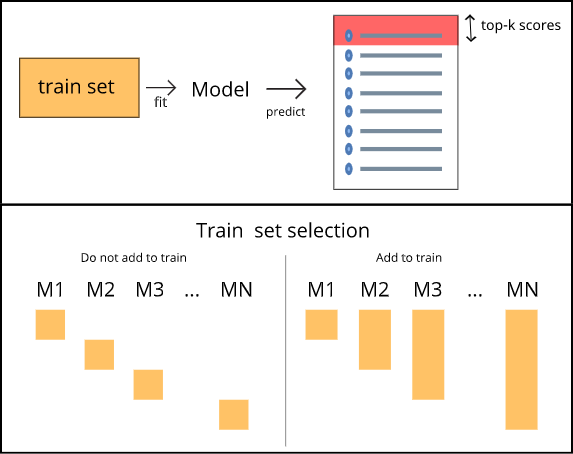
\includegraphics[scale=0.72]{Images/image1.png}
    \caption{Two ways of treating the train set in iterative algorithm}
    \label{TrainSetSelection}
\end{figure}

In iterative algorithms, only regression methods were used.
The pipeline of the algorithm consists of the following steps:
\begin{enumerate}
    \item In the initial step, a predefined number of molecules are docked or taken from the list of already docked compounds to provide a test set;
    \item The ML model is trained and integrated then into a complex model;
    \item The complex model predicts the docking outcome;
    \item The batch of molecules is docked: if the number of docking hits is larger than a predefined size, then the demanded number of hits are sampled;
    In the opposite situation, randomly sampled molecules from non-hits are added to all docking hits in order to gain the required amount;
    \item Depending on the algorithm protocol (Fig. \ref{TrainSetSelection}), the batch from the precious step is either added to the train dataset, or is utilized as a train dataset itself;
    \item Steps 2-5 are repeated until the predetermined number of iteration is reached.
\end{enumerate}

\subsection{Train set selection}
There are two ways to update train dataset from iteration to iteration (Fig. \ref{TrainSetSelection}).
On the one hand, it is profitable to make use of all the docked molecules, because more information is gathered.
Most likely that single models in one round of iteration algorithm will be similar to each other and prioritize the molecules which properties close to each other.
On the other hand, the selection of only the latest batch of docked molecules for training may cause more diversity in single models' parameters.
Thus, models from different step will search for docking hits in various parts of chemical space.
Both approaches were tested within the iterative algorithms.\\

\subsection{Complex model creation}


\begin{figure}
    \centering
    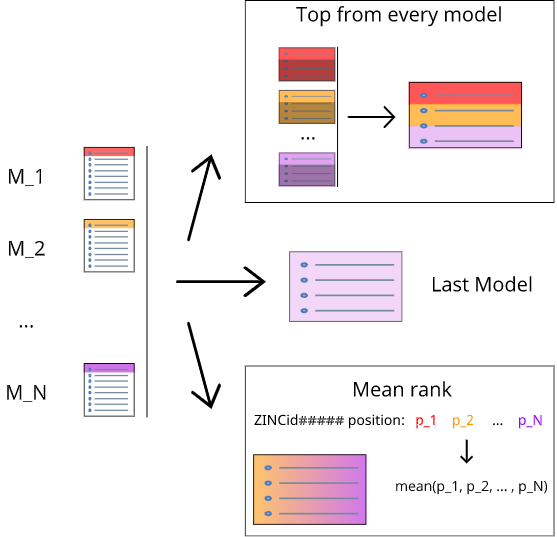
\includegraphics[scale=0.8]{Images/image2.png}
    \caption{Types of complex model}
    \label{ComplexModels}
\end{figure}

If there are several ML models available, it is possible to combine them somehow to create a complex model.
Three types of complex models were employed in the algorithm (Fig. \ref{ComplexModels}):
\begin{itemize}
    \item \textbf{Last Model}: ML model from the latest iteration is treated as a complex model and used to predict docking outcomes.
    After the prediction, top-k\% of predicted scores become hits;
    \item \textbf{Top from every model}: on the $\text{n}^{th}$ iteration, each model makes a prediction and top-(k/n)\% of predicted scores from each model constitute complex model's hits (repetitions are deleted);
    \item \textbf{Mean Rank}: for each compound, the positions in the ratings of all models are averaged; the k\% of the compounds with the smallest average positions are handled as hits.
\end{itemize}


\section{Linear model visualisation}
If complex model is composed of linear regressions, the coefficients of single models can be visualised with help of t-SNE, t-distributed stochastic neighbor embedding.
This visualisation can help to analyse whether single models in the iterative algorithm are diverse or not. \\

The coefficients of linear regression models were normalised so the sum of their squares was equal 1.
TSNE algorithm from scikit-learn library was utilised to project the 2048-dimensional space of coefficients to 2D space. 

